\begin{figure}[t!]
\small
\begin{center}
\setlength{\tabcolsep}{1pt}
\begin{tabular}{cccc}
\hspace{3mm} Task OSSE & 
 Task OSSE & 
\hspace{-10mm} Task OSSE & 
\hspace{-10mm}Task OSE \\
\hspace{3mm}  Nadir & 
 Nadir + SWOT & 
\hspace{-10mm} Nadir + SST & 
\hspace{-10mm}Nadir \\
%\vspace{-2mm}
%%%%% SSH %%%%%%%%
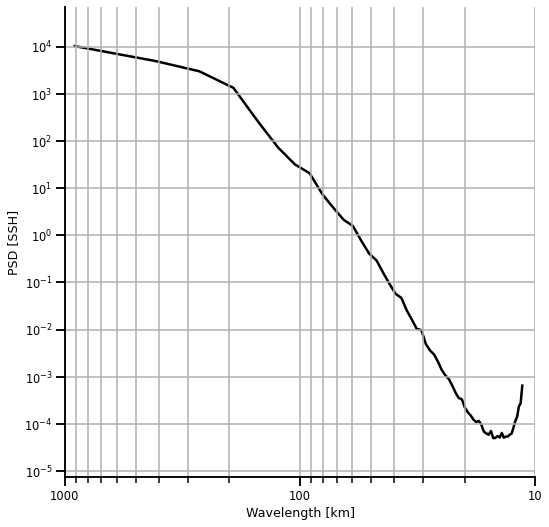
\includegraphics[trim={0 0 0 0},clip, width=3.70cm,height=3.5cm]{00_Oceanbench/content/figures/fourdvarnet_figs/osse_gf_nadir_isotrop.png} &
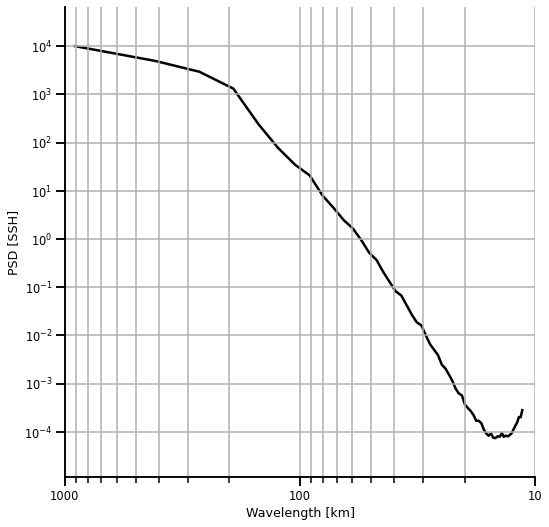
\includegraphics[trim={18mm 0 0 0},clip, width=3.3cm,height=3.5cm]{00_Oceanbench/content/figures/fourdvarnet_figs/osse_gf_nadirswot_isotrop.png} &
\hspace{-5mm}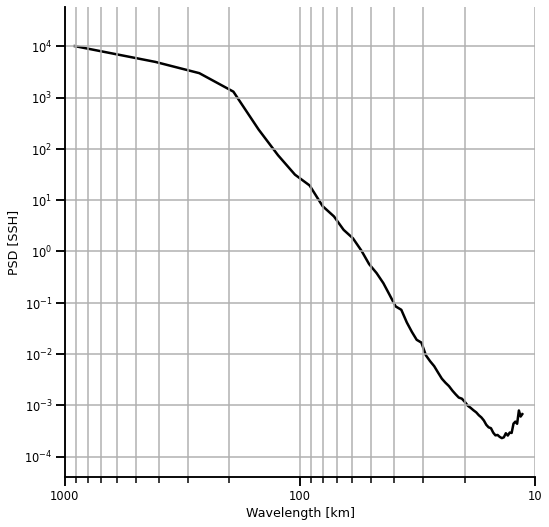
\includegraphics[trim={18mm 0 0 0},clip, width=3.3cm,height=3.5cm]{00_Oceanbench/content/figures/fourdvarnet_figs/osse_gf_nadir_sst_isotrop.png} &
\hspace{-10mm}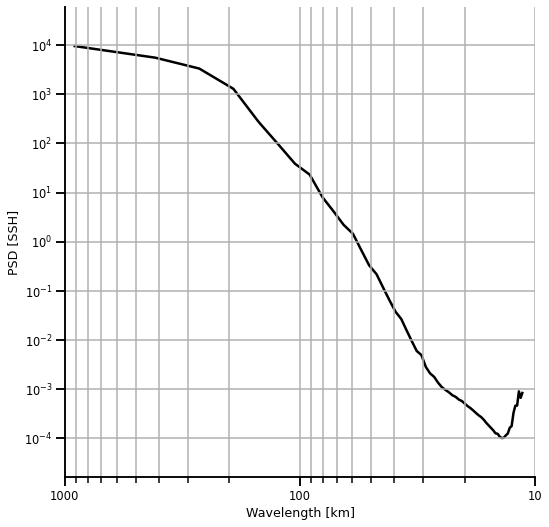
\includegraphics[trim={18mm 0 0 0},clip,width=3.3cm,height=3.5cm]{00_Oceanbench/content/figures/fourdvarnet_figs/ose_gf_isotrop.png} \\
%\vspace{3mm}
%%%%% KINETIC ENERGY %%%%%%%%
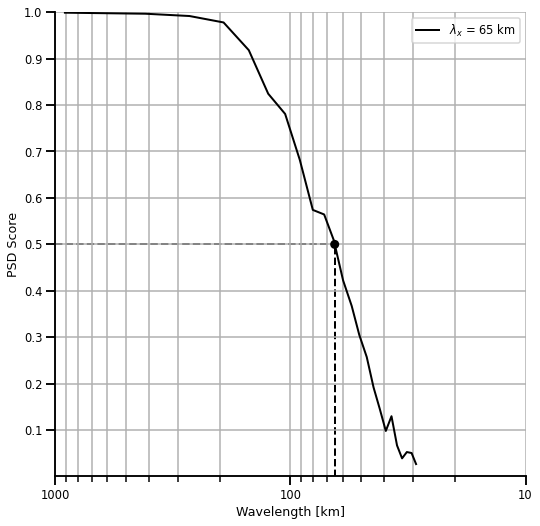
\includegraphics[trim={0 0 0 0}, clip, width=3.70cm,height=3.5cm]{00_Oceanbench/content/figures/fourdvarnet_figs/osse_gf_nadir_1d_psd_score.png} &
\hspace{1mm}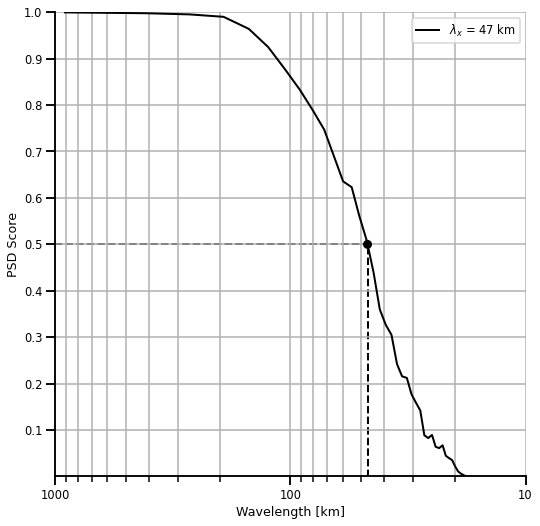
\includegraphics[trim={18mm 0 0 0},clip, width=3.3cm,height=3.5cm]{00_Oceanbench/content/figures/fourdvarnet_figs/osse_gf_nadirswot_1d_psd_score.png} &
\hspace{-4mm}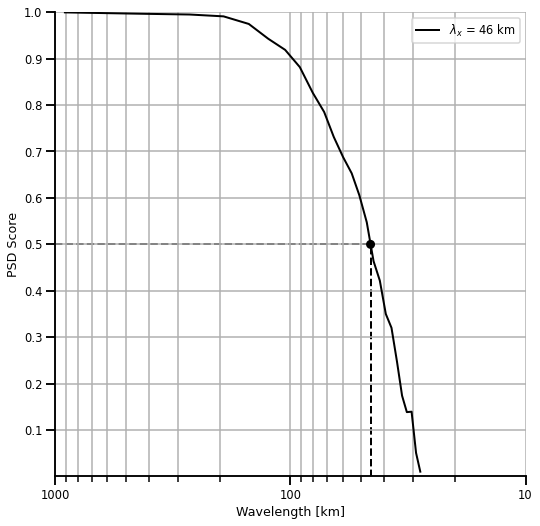
\includegraphics[trim={18mm 0 0 0},clip, width=3.3cm,height=3.5cm]{00_Oceanbench/content/figures/fourdvarnet_figs/osse_gf_nadir_sst_1d_psd_score.png} &
\hspace{-10mm}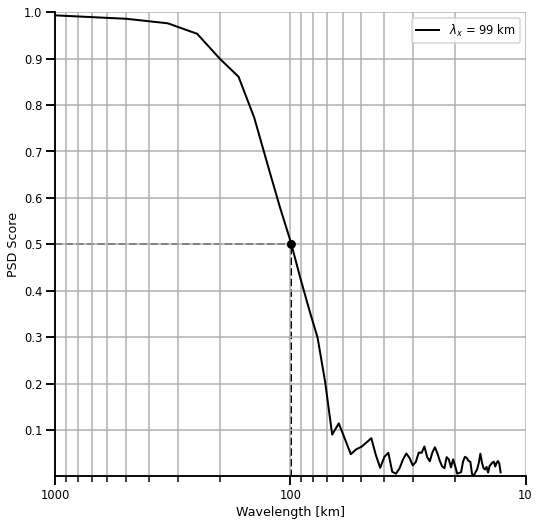
\includegraphics[trim={18mm 0 0 0},clip,width=3.3cm,height=3.5cm]{00_Oceanbench/content/figures/fourdvarnet_figs/ose_gf_1d_psd_score.png} \\
%%%%% RELATIVE VORTICITY %%%%%%%%
\hspace{-4mm}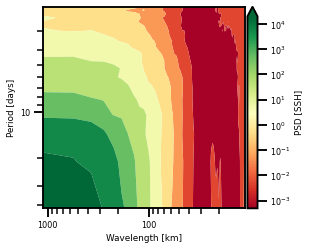
\includegraphics[trim={0 0 23mm 0},clip, width=3.65cm,height=3.5cm]{00_Oceanbench/content/figures/fourdvarnet_figs/osse_gf_nadir_psd_spacetime.png} &
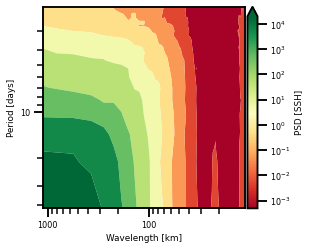
\includegraphics[trim={14mm 0 23mm 0},clip, width=3cm,height=3.5cm]{00_Oceanbench/content/figures/fourdvarnet_figs/osse_gf_nadirswot_psd_spacetime.png} &
\hspace{-5mm}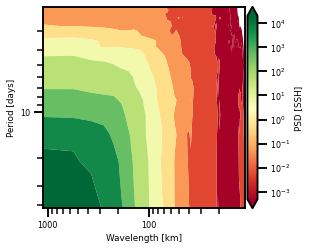
\includegraphics[trim={14mm 0 23mm 0},clip, width=3cm,height=3.5cm]{00_Oceanbench/content/figures/fourdvarnet_figs/osse_gf_nadir_sst_psd_spacetime.png} &
\hspace{-5mm}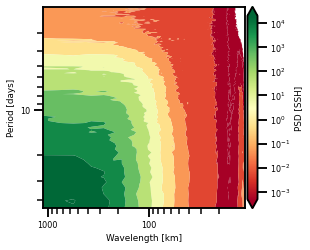
\includegraphics[trim={14mm 0 0 0},clip,width=3.8cm,height=3.5cm]{00_Oceanbench/content/figures/fourdvarnet_figs/ose_gf_psd_spacetime.png} \\
%%%%% STRAIN %%%%%%%%
\hspace{-4mm}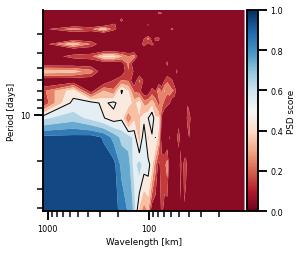
\includegraphics[trim={0 0 23mm 0},clip, width=3.70cm,height=3.5cm]{00_Oceanbench/content/figures/fourdvarnet_figs/osse_gf_nadir_psd_spacetime_score.png} &
\hspace{-2mm}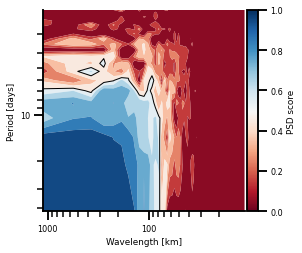
\includegraphics[trim={13mm 0 23mm 0},clip, width=3.1cm,height=3.5cm]{00_Oceanbench/content/figures/fourdvarnet_figs/osse_gf_nadirswot_psd_spacetime_score.png} &
\hspace{1mm}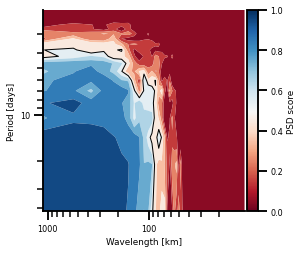
\includegraphics[trim={13mm 0 0 0},clip, width=3.8cm,height=3.5cm]{00_Oceanbench/content/figures/fourdvarnet_figs/osse_gf_nadir_sst_psd_spacetime_score.png} &
 \\
% \vspace{-2mm}
 \hspace{1mm} (a) & \hspace{-5mm} (b) & \hspace{-8mm}(c) & \hspace{-10mm}(d)
\end{tabular}
\vspace{-3mm}
% \caption{Row I - Isotrophic PSD. Row 2 - Isotrophic PSD Score}
\caption{
Power spectrum and associated scores of the 4dVarNet method for each of the four tasks.
The row display in order: (1) the isotropic PSD, (2) the spatial PSD score (using the isotropic PSD for the first three rows and along track PSD for the last row), (3) the space-time PSD, (4) The spacetime PSD score available only in OSSE task.  }

\vspace{-5mm}
\label{fig:oceanbench_psd_4dvarnet}
\end{center}
\end{figure}
